\documentclass[handout]{beamer}

\beamertemplatenavigationsymbolsempty


\mode<presentation>
{
\usetheme[width=0cm]{Goettingen}
\usecolortheme{seahorse}
\useoutertheme{SEFM}
}

\input{header}
\usepackage[english]{babel}
% or whatever

\usepackage[utf8x]{inputenc}

\usepackage{times}
\usepackage[T1]{fontenc}


% Or whatever. Note that the encoding and the font should match. If T1
% does not look nice, try deleting the line with the fontenc.

\usepackage{pgf,tikz}
\usetikzlibrary{decorations}
\usetikzlibrary{arrows}
\usetikzlibrary{shapes.arrows}
\usetikzlibrary{shapes.multipart}

\usepackage{url}

%% Define a new 'leo' style for the package that will use a smaller font.
\makeatletter
\def\url@leostyle{%
  \def\UrlFont{\sf\small}}
\makeatother
%% Now actually use the newly defined style.
\urlstyle{leo}

\lstdefinelanguage{Smalltalk}{
  basicstyle=\ttfamily,
  keywordstyle=\bfseries,
  morekeywords={self,super,true,false,nil,thisContext}, % This is overkill
  morestring=[d]',
  morecomment=[s]{"}{"},
  alsoletter={\#:},
  escapechar={!},
}[keywords,comments,strings]


\newcommand{\Blue}[1]{\color{blue}#1\color{black}}

\title[OOP]{Object-Oriented Programming}

\subtitle[Inheritance, Reuse etc.]{OO: Inheritance, Code Reuse and Multi-Dispatch}


\author[Richard Bubel] % (optional, use only with lots of authors)
{Richard Bubel \\ based on slides from Sibylle Schupp and Jean-Philippe Bernardy}
% - Use the \inst{?} command only if the authors have different
%   affiliation.

% - Use the \inst command only if there are several affiliations.
% - Keep it simple, no one is interested in your street address.

\institute[CTH]{Chalmers University of Technology}

\date{25th November 2010}%[Short Occasion] % (optional)


\subject{Talks}
% This is only inserted into the PDF information catalog. Can be left
% out.



% If you have a file called "university-logo-filename.xxx", where xxx
% is a graphic format that can be processed by latex or pdflatex,
% resp., then you can add a logo as follows:

%\pgfdeclareimage[height=0.5cm]{university-logo}{../../../project/gitroot/clipart/ChalmGUmarke.pdf}
% \logo{\pgfuseimage{university-logo}}


\begin{document}
\begin{frame}
  \titlepage
\end{frame}

\begin{frame}[fragile]
\frametitle{References}
References:
\begin{itemize}
\item M. Scott, Programming Language Pragmatics

\url{http://www.cs.rochester.edu/u/scott/254/notes/09-objects}
\item K. Loudon, Programming Languages---Principles and Practice
(not on-line available)
\end{itemize}

Additional reading:
\begin{itemize}
\item B. Ryders, Univ. Rutgers
\url{
http://remus.rutgers.edu/cs314/s2004/ryder/lectures/adt-15Newest-2up.pdf
}
%
\item K. Bruce, Williams College
\url{
http://www.cs.williams.edu/~kim/cs334/s00/Lectures/Lec13/Lec13.html}
\end{itemize}
\end{frame}

\begin{frame}[fragile]
\frametitle{Smalltalk Introduction}
The next slides about ST are repeated from last lecture as we did not
completely finish the walk-through. 
\end{frame}



\section{Smalltalk Introduction}

\begin{frame}[fragile]
\frametitle{Smalltalk Introduction}

Smalltalk is a \emph{single paradigm} language, i.e.,
\begin{itemize}
  \item \emph{no} primitive types 
  \item \emph{everything} is an object, incl.\ integer
    literals (\texttt{1},\texttt{2} etc.), character literals etc.
  \item \emph{strict} data encapsulation:
    \begin{itemize}
    \item all fields are private
    \item objects communicate solely via \emph{messages}
    \end{itemize}
\end{itemize}

\bigskip\pause

Smalltalk comes with an IDE built-in.

\bigskip

We use Squeak (\url{http://www.squeak.org})

\begin{itemize}
  \item Good introduction into Smalltalk: \url{http://stephane.ducasse.free.fr/FreeBooks/ByExample/SmalltalkByExampleNewRelease.pdf}
  \item Good Squeak specific free book: \url{http://www.squeakbyexample.org/}
\end{itemize}

\end{frame}


%%%%%%%%%%%%%%%%%%%%%%%%%%%%%%%%%%%%%%%%%%%%%%%

\begin{frame}[fragile]
  \frametitle{Classes in Smalltalk}

Class Declaration:

\begin{lstlisting}[language=Smalltalk]
!\textit{NameOfSuperClass}! subclass: #!\textit{NameOfSubclass}!
  !\color<2>{red}\texttt{instanceVariableNames}!: ''!\color{black}!
  !\color<3>{red}\texttt{classVariableNames}!: ''!\color{black}!
  poolDictionaries: ''!\color{black}!
  !\color<4>{red}\texttt{category}!: ''
\end{lstlisting}

\begin{itemize}
\item '$\langle some\_text\rangle$' String literal
\item \#$\langle some\_name\rangle$ (Instance of) Symbol of given name
\item<2-> \texttt{instanceVariableNames} 
 \begin{itemize} 
    \item space separated list of instance field names, e.g., 'day month year'
    \item fields (variables) are untyped
    \item fields (variables) contain references to objects (like in Java)      
  \end{itemize}
\item<3-> \texttt{classVariableNames} (class/static fields; otherwise similar)
\item<4-> \texttt{category}: Classes are loosely organized in categories
  (attention: no semantics, i.e., do not declare namespace or similar)  
\end{itemize}

%% Demo

\end{frame}


%%%%%%%%%%%%%%%%%%%%%%%%%%%%%%%%%%%%%%%%%%%%%%%

\begin{frame}[fragile]
  \frametitle{Object Creation}

  Objects are instantiated by sending the class object the message \texttt{new}

\begin{lstlisting}[language=Smalltalk]
   MyClass new
\end{lstlisting}

\begin{itemize}
  \item allocates memory
  \item instance fields are set to \texttt{nil} (attention:
    \texttt{nil} is an object itself)
  \item (reference to) newly created object returned
\end{itemize}

\pause\bigskip

\emph{No} explicit initialization. By convention \emph{only}:
\begin{itemize}
  \item objects implement a method \texttt{initialize} called
    explicitly after creation.
  \item lazy initialization: trigger initialization within
    getter (accessor) method
\end{itemize}

\end{frame}

%%%%%%%%%%%%%%%%%%%%%%%%%%%%%%%%%%%%%%%%%%%%%%%

\begin{frame}[fragile]
\frametitle{Messages and methods}

\begin{lstlisting}[language=Smalltalk]
messageSelectorAndArgumentNames
  "comment stating purpose of message"

  | temporary variable names |
  statements
\end{lstlisting}

In Smalltalk messages/methods have
\begin{itemize}
  \item implicit parameter \texttt{self}
  \item always a return value
    \begin{itemize}
      \item explicit: \texttt{\^}\textit{expr}
      \item implicit (if no explicit given): callee (\texttt{self} object) returned
   \end{itemize}
 \item parameter passing: copy-by-value (as in Java; attention:
   references to objects are copied \emph{not objects})
 \item single dynamic dispatch
\end{itemize}

\end{frame}

%%%%%%%%%%%%%%%%%%%%%%%%%%%%%%%%%%%%%%%%%%%%%%%

\begin{frame}[fragile]
\frametitle{Messages and methods: Invocation}

\begin{example}
\begin{lstlisting}[language=Smalltalk]
setDate:aYear month:aMonth day:aDay 
  "sets a specific date"

  year  := aYear.
  month := aMonth.
  day   := aDay
\end{lstlisting}
\end{example}

Invocation:
\lstinline[language=Smalltalk]+ myDateObj setDate:2010 month:11 day:19+

\pause\bigskip

What is returned? \pause \texttt{myDateObj}

\end{frame}

%%%%%%%%%%%%%%%%%%%%%%%%%%%%%%%%%%%%%%%%%%%%%%%

\begin{frame}[fragile]
\frametitle{Special Messages}


\Blue{Arithmetic Messages and Comparison}:

Message `+`: \texttt{1 + 3}

\begin{itemize}
\item Who is the callee (receiver) object? \pause \texttt{1}\\
  The object \texttt{1} receives the message \texttt{+} with argument \texttt{3}.
\item Similar: \texttt{ -,*,/,\ldots,<,>,\ldots}
\item Evaluation order from left to right:
  \begin{itemize}
    \item Result of \texttt{1 + 2 * 3}? \pause \alert{\texttt{9}}
  \end{itemize}
\end{itemize}

\Blue{Equality}

\begin{itemize}
\item \texttt{x == y}: reference equality (is receiver object and
  argument the same object) (negation: \verb+~~+)
\item \texttt{x = y}: equality (same as Java's equals method, must be
  defined by user) (negation: \verb+~=+)
\end{itemize}
\pause

All can be overridden by the user!

\end{frame}

%%%%%%%%%%%%%%%%%%%%%%%%%%%%%%%%%%%%%%%%%%%%%%%

\begin{frame}[fragile]
\frametitle{Statements: Assignment, Concatenation}

\Blue{Assignment}: Reference semantics as for Java (in case of objects)
\begin{center}
\textit{fieldOrVar} \alert{\texttt{:=}} \textit{expr}
\end{center}

\pause\bigskip

\Blue{Concatenation of Statements}

\begin{center}
\textit{stmnt1}{\huge\alert{\texttt{.}}}\textit{stmnt2}
\end{center}

\end{frame}


%%%%%%%%%%%%%%%%%%%%%%%%%%%%%%%%%%%%%%%%%%%%%%%

\begin{frame}[fragile]
\frametitle{Statements: Method invocations}

\Blue{Call chains}

\begin{itemize}
\item<1->
\begin{lstlisting}[language=Smalltalk]
result := (list add: 1) add: 2
\end{lstlisting} 
in Java: \texttt{result = list.add(1).add(2)} (Attention: in Smalltalk
\texttt{add} on collections returns added object; so above will most
likely not be what you want. Why? \onslide<2-> triggers error resp.\ 
if Integer would provide \texttt{add} \texttt{result} assigned the value \texttt{3}) 
\item<2-> 
\begin{lstlisting}[language=Smalltalk]
(result := list) add: 1; add: 2
\end{lstlisting} 
the semicolon \texttt{;} sends message to receiver of previous
message. The above statement assigns \texttt{result} the list (1,2) as intended.

\end{itemize}

\onslide<3->

\Blue{Method not understood}

Sending a message to an object for which it does not have a method
causes a \texttt{MethodNotUnderstood} exception.


\end{frame}

%%%%%%%%%%%%%%%%%%%%%%%%%%%%%%%%%%%%%%%%%%%%%%%

\begin{frame}[fragile]
\frametitle{Statements: Selection and Code Blocks}

Realized as methods of \texttt{Boolean} class

\begin{lstlisting}[language=Smalltalk]
  (1 < 2) ifTrue: [j := 1] ifFalse: [j := 2]
\end{lstlisting} 

\pause\medskip

\begin{block}{Code blocks [ ... ]}
\emph{Code blocks} are objects themselves. They
\begin{itemize}
  \item consist of a sequence of statements
  \item are evaluated when message \texttt{value} received
  \item may have parameters: 
    \lstinline[language=Smalltalk]{[ :param | ... ]} \\
    evaluation triggered by \texttt{value: aValue}
\end{itemize}

\end{block}


\end{frame}

%%%%%%%%%%%%%%%%%%%%%%%%%%%%%%%%%%%%%%%%%%%%%%%

\begin{frame}[fragile]
\frametitle{Loops: While and For-Loops}

\Blue{Loops}\medskip

Defined as methods of code blocks:

\begin{lstlisting}[language=Smalltalk]
   [ i>=0 ] whileTrue: [ doSomething ]
   [ i<0 ] whileFalse: [ doSomething ]

  1 to: 10 by: 2 do: [: i | Transcript show: i; cr].
  5 timesRepeat [ doSomething ]   
\end{lstlisting} 

\end{frame}

%%%%%%%%%%%%%%%%%%%%%%%%%%%%%%%%%%%%%%%%%%%%%%%

\begin{frame}[fragile]
\frametitle{Arrays}

\Blue{Arrays}\medskip

\begin{lstlisting}[language=Smalltalk]
|array| 
  array := #( 1 2 3) "creates an array of literals"
  do: [:each | Transcript show: each] 
\end{lstlisting} 



\begin{lstlisting}[language=Smalltalk]
 "creates array of size 10;"
     "can be populated with non literals"
 array := IntegerArray new: 10. 
 array at:0 put:1;at:2 put: 4711.
 array do: [:each | Transcript show: each] 
  
\end{lstlisting} 

\end{frame}

\section{Back to inheritance: An imperfect world}

\subsection{Multiple Inheritance}
\begin{frame}[fragile]
\begin{center}\Huge Code-Reuse\end{center}
\end{frame}

\begin{frame}[fragile]
\frametitle{Motivation--First Example}
\framesubtitle{}
Consider the following classes (cp. Smalltalk)
\begin{itemize}
\item Magnitude: for objects that are measurable (comparable)
\item Number: for objects that are measurable and have arithmetics
\end{itemize}
Assume you want to add the classes Char, Integer, and Complex.
Constraints
\begin{itemize}
\item Char should be subclass of Magnitude, but not of Number.
\item Integer should be subclass of Magnitude and Number.
\item Complex should be a subclass of Number, but not of Magnitude.
\end{itemize}
Impossible with single inheritance.
\end{frame}

\begin{frame}[fragile]
\frametitle{Limitations of single inheritance}
\framesubtitle{}
Workarounds for the previous example:

\begin{itemize}
\item Limit inheritance: eliminate class Magnitude; every measurable
class implements its comparisons
\item Violate substitutability: define Complex as subclass of Number
(and Number as subclass of Measurable), but override measurable
methods so that they trigger error.
\item Avoid inheritance: define each method in each of the classes
Char, Integer, Complex.
\end{itemize}
\end{frame}

\begin{frame}[fragile]
\frametitle{Motivation: A Second Example}
\framesubtitle{}
\begin{overlayarea}{\textwidth}{\textheight}\centering
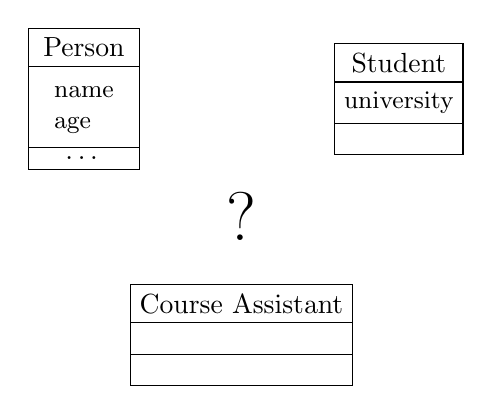
\begin{tikzpicture}
  \node[draw, rectangle split, rectangle split parts=3] (Person)   at
  (0,0) {Person \nodepart{second}\small \begin{tabular}{l}name\\
      age\end{tabular}
    \nodepart{third}
    \ldots
 };
  \node[draw, rectangle split, rectangle split parts=3] (Student)  at (4,0){Student
    \nodepart{second} \small university
 };
\only<2>{
 \node[draw, rectangle split, rectangle split parts=3] (CA) at (2,-3) {Course Assistant};
  \node[] (CA) at (2,-1.5) {\Huge  \alert{?}};
}
\end{tikzpicture}
\end{overlayarea}
\vfill
\end{frame}

\begin{frame}[fragile]
\frametitle{Take 1: Multiple Inheritance}
\framesubtitle{}
\begin{overlayarea}{\textwidth}{0.55\textheight}\centering
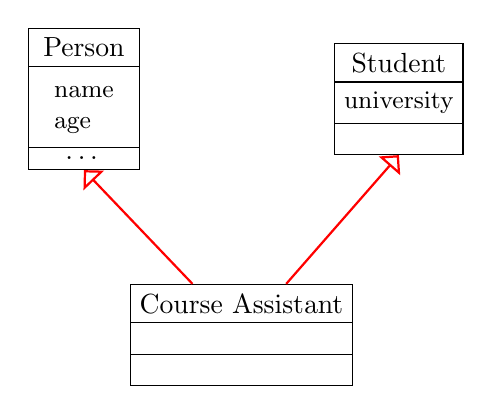
\begin{tikzpicture}
  \node[draw, rectangle split, rectangle split parts=3] (Person)   at
  (0,0) {Person \nodepart{second}\small \begin{tabular}{l}name\\
      age\end{tabular}
    \nodepart{third}
    \ldots
 };
  \node[draw, rectangle split, rectangle split parts=3] (Student)  at (4,0){Student
    \nodepart{second} \small university
 };
\node[draw, rectangle split, rectangle split parts=3] (CA) at (2,-3) {Course Assistant
};

\draw[color=red, thick, open triangle 90-] (Person.south) -- (CA);
\draw[color=red, thick, open triangle 90-] (Student.south) -- (CA);

\end{tikzpicture}
\end{overlayarea}

\Blue{Multiple Inheritance}

\qquad A class may inherit from \alert{one or more} superclasses.
\pause\medskip

\Blue{Languages}
\begin{itemize}
\item Most OO languages support single inheritance only.
\item Eiffel, \cpp, CLOS support multiple inheritance.
\item Java, C\# support ``interfaces''. 
\end{itemize}
\end{frame}

\begin{frame}[fragile]
\frametitle{Object model under multiple inheritance}
\framesubtitle{}
\begin{tabular}{ll}
\begin{minipage}{4.3cm}
\begin{cplus3}
class Person
{ 
   int p1;
   int& p2;
   boolean p3; 
   virtual void m1(..) {...}
   virtual int m2(..) {...}  
};
class Student 
{
   char s1;
   char s2;
};
class Asst : Person, Student 
{
    int a1;
};
\end{cplus3}
\end{minipage}

& 

\begin{tabular}{l}
{\small 
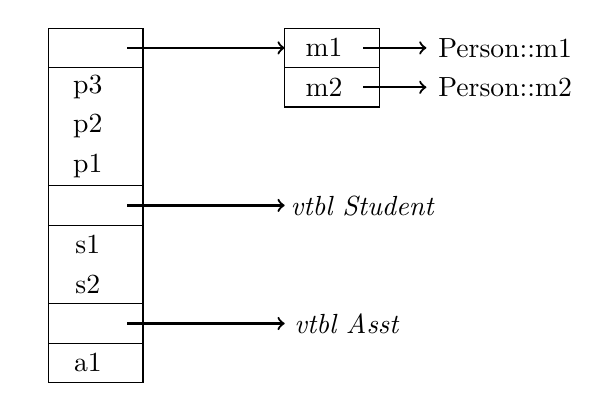
\begin{tikzpicture}

% object 3
\draw (0,-2.5)  rectangle (1.2,-3.0);
\pgftext[at={\pgfpoint{0.5cm}{-2.75cm}}]{a1} ;

% vptr object 3
\draw (0,-2.5)  rectangle (1.2,-2.0);
\pgftext[at={\pgfpoint{0.5cm}{-2.25cm}}]{} ;
\draw[->, thick] (1.0, -2.25) -- (3.0,-2.25); 
\pgftext[at={\pgfpoint{3.8cm}{-2.25cm}}]{\textit{vtbl Asst}} ;

% object 2
\draw (0,-2.0)  rectangle (1.2,-1.0);
\pgftext[at={\pgfpoint{0.5cm}{-1.25cm}}]{s1} ;
\pgftext[at={\pgfpoint{0.5cm}{-1.75cm}}]{s2} ;

% vptr
\draw (0,-1.0)  rectangle (1.2,-0.5);
\pgftext[at={\pgfpoint{-0.25cm}{-0.75cm}}]{} ;
\draw[->, thick] (1.0, -0.75) -- (3.0,-0.75); 
\pgftext[at={\pgfpoint{4.0cm}{-0.75cm}}]{\textit{vtbl Student}} ;

% object 1
\pgftext[at={\pgfpoint{0.5cm}{-0.25cm}}]{p1} ;
\pgftext[at={\pgfpoint{0.5cm}{0.25cm}}]{p2} ;
\pgftext[at={\pgfpoint{0.5cm}{0.75cm}}]{p3} ;
\draw (0,-0.5)  rectangle (1.2,1.5);

% vptr 
\draw (0,1.0)  rectangle (1.2,1.5);
\pgftext[at={\pgfpoint{0.5cm}{1.25cm}}]{} ;
\draw[->, thick] (1.0, 1.25) -- (3.0,1.25); 





% right one 

% vtbl for 

% vtbl for Person
%\draw (3,-0.5)  rectangle (4.2,0.0);
%\pgftext[at={\pgfpoint{3.5cm}{-0.25cm}}]{m4} ;
%\draw[->, thick] (4.0, -0.25) -- (4.8,-0.25); 
%\pgftext[at={\pgfpoint{5.8cm}{-0.25cm}}]{Person::m4} ;


%\draw (3,0)  rectangle (4.2,0.5);
%\pgftext[at={\pgfpoint{3.5cm}{0.25cm}}]{m3} ;
%\draw[->, thick] (4.0, 0.25) -- (4.8,0.25); 
%\pgftext[at={\pgfpoint{5.8cm}{0.25cm}}]{Person:m3} ;

\draw (3,0.5)  rectangle (4.2,1.0);
\pgftext[at={\pgfpoint{3.5cm}{0.75cm}}]{m2} ;
\draw[->, thick] (4.0, 0.75) -- (4.8,0.75); 
\pgftext[at={\pgfpoint{5.8cm}{0.75cm}}]{Person::m2} ;

\draw (3,1.0)  rectangle (4.2,1.5);
\pgftext[at={\pgfpoint{3.5cm}{1.25cm}}]{m1} ;
\draw[->, thick] (4.0, 1.25) -- (4.8,1.25); 
\pgftext[at={\pgfpoint{5.8cm}{1.25cm}}]{Person::m1} ;

\end{tikzpicture}
}
\end{tabular}

\end{tabular}

\end{frame}


\begin{frame}[fragile]
\frametitle{\only<1>{Great, solves our problem!}\only<2->{Problem: Name Clashes}}
\framesubtitle{}
\begin{overlayarea}{\textwidth}{0.55\textheight}\centering
\begin{tikzpicture}
  \node[draw, rectangle split, rectangle split parts=3] (Person)   at
  (0,0) {Person \nodepart{second}\small \begin{tabular}{l}\alert<2->{name}\\
      age\only<2->{\\ \alert{id} }\end{tabular}
    \nodepart{third}
    \ldots
 };
  \node[draw, rectangle split, rectangle split parts=3] (Student)  at (4,0){Student
    \nodepart{second} \small \begin{tabular}{l} university \only<2->{\\ \alert{name} \\ \alert{id}} \end{tabular}
 };
\node[draw, rectangle split, rectangle split parts=3] (CA) at (2,-3) {Course Assistant
};

\draw[thick, open triangle 90-] (Person.south) -- (CA);
\draw[thick, open triangle 90-] (Student.south) -- (CA);

\end{tikzpicture}
\end{overlayarea}

\end{frame}


\begin{frame}[fragile]
\frametitle{Name Clashes: Conflict Resolutions}
\framesubtitle{}

If two base classes define a method or field of same signature,
the ambiguity must be resolved. 

\medskip

\begin{itemize}
\item<+-> Language-defined priorities, e.g., CLOS: first-fit
\item<+-> Prohibited (and checked), e.g., Eiffel
\begin{itemize}
\item Compile-time error (of child class) must be resolved manually,
  e.g., via \texttt{rename}, \texttt{select}, etc.
\begin{eiffel}
class COURSE_ASSISTANT
inherit
      STUDENT
          rename
              name as teacher_name
              id   as student_id
          end
      PERSON
\end{eiffel}
\end{itemize}
\item<+-> Ambiguous \alert{use} prohibited (and checked)
\begin{itemize}
\item \Cpp: no error at class compilation time, but at method invocation
time (statically)
\item Must be resolved manually,  via scope resolution operator
\begin{cplus3}
if (...) person::name() else student::name(); 
\end{cplus3} 
\end{itemize}
\end{itemize}
\end{frame}


\begin{frame}[fragile]
\frametitle{OK, that's all? Let's do it  so.}
\framesubtitle{}
\begin{overlayarea}{\textwidth}{0.55\textheight}\centering
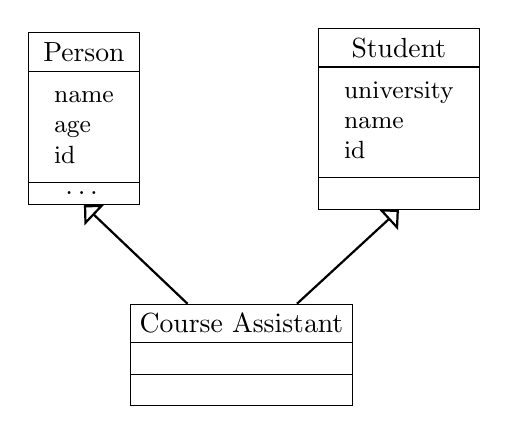
\begin{tikzpicture}
  \node[draw, rectangle split, rectangle split parts=3] (Person)   at
  (0,0) {Person \nodepart{second}\small \begin{tabular}{l}name \\
      age\\ id \end{tabular}
    \nodepart{third}
    \ldots
 };
  \node[draw, rectangle split, rectangle split parts=3] (Student)  at (4,0){Student
    \nodepart{second} \small \begin{tabular}{l} university \\ name \\ id \end{tabular}
 };
\node[draw, rectangle split, rectangle split parts=3] (CA) at (2,-3) {Course Assistant
};

\draw[thick, open triangle 90-] (Person.south) -- (CA);
\draw[thick, open triangle 90-] (Student.south) -- (CA);
\end{tikzpicture}
\end{overlayarea}

\end{frame}

\begin{frame}{Problem: Repeated Inheritance}
\begin{minipage}{0.5\textwidth}
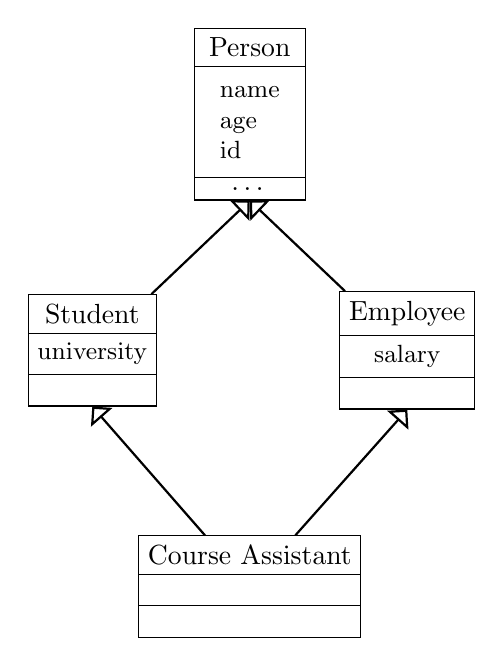
\begin{tikzpicture}
  \node[draw, rectangle split, rectangle split parts=3] (Person)   at
  (0,3) {Person \nodepart{second}\small \begin{tabular}{l}name\\
      age\\ id\end{tabular}
    \nodepart{third}
    \ldots
 };
  \node[draw, rectangle split, rectangle split parts=3] (Student)  at (-2,0){Student
    \nodepart{second} \small university
 };
  \node[draw, rectangle split, rectangle split parts=3] (Employee) at
  (2,0) {Employee
    \nodepart{second} \small salary    
  };
  \node[draw, rectangle split, rectangle split parts=3] (CA) at (0,-3) {Course Assistant}; 
\only<2>{\color{red}}
 \draw[thick, open triangle 90-] (Person.south) -- (Student);
 \draw[thick, open triangle 90-] (Student.south) -- (CA);
\only<2>{\color{blue}}
  \draw[thick, open triangle 90-] (Person.south) -- (Employee);
 \draw[thick, open triangle 90-] (Employee.south) -- (CA);
\end{tikzpicture}
\end{minipage}
\begin{minipage}{0.49\textwidth}
  \onslide<2->
  \begin{block}{Repeated Inheritance}
    A class serves as ancestor repeatedly through multiple
    inheritance paths.
  \end{block} \vfill
  \onslide<3->
  \emph{Which semantics are possible?}
  \onslide<4->
  \begin{itemize}
    \item \Blue{Replicated Inheritance}: \texttt{Course Assistant}
      contains two copies of \texttt{Person} (default in \cpp) 
    \item \Blue{Shared Inheritance (``diamond'')}: \texttt{Course
        Assistant} contains only 1 object (Eiffel, \cpp via keyword \texttt{virtual}).
 \end{itemize}

\end{minipage}

\end{frame}


\begin{frame}{Replicated Inheritance}
\begin{minipage}{0.5\textwidth}
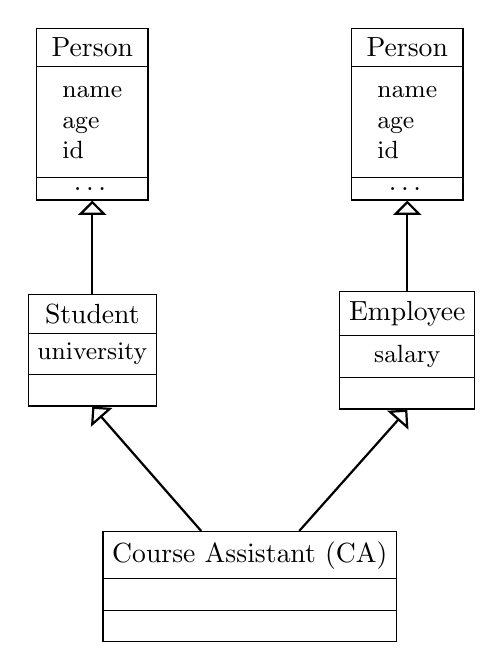
\begin{tikzpicture}
  \node[draw, rectangle split, rectangle split parts=3] (PersonViaS)   at
  (-2,3) {Person \nodepart{second}\small \begin{tabular}{l}name\\
      age\\ id\end{tabular}
    \nodepart{third}
    \ldots
 };
  \node[draw, rectangle split, rectangle split parts=3] (PersonViaE)   at
  (2,3) {Person \nodepart{second}\small \begin{tabular}{l}name\\
      age\\ id\end{tabular}
    \nodepart{third}
    \ldots
 };
 \node[draw, rectangle split, rectangle split parts=3] (Student)  at (-2,0){Student
    \nodepart{second} \small university
 };
  \node[draw, rectangle split, rectangle split parts=3] (Employee) at
  (2,0) {Employee
    \nodepart{second} \small salary    
  };
  \node[draw, rectangle split, rectangle split parts=3] (CA) at (0,-3)
  {Course Assistant (CA)}; 
\draw[thick, open triangle 90-] (PersonViaS.south) -- (Student);
 \draw[thick, open triangle 90-] (Student.south) -- (CA);
 \draw[thick, open triangle 90-] (PersonViaE.south) -- (Employee);
 \draw[thick, open triangle 90-] (Employee.south) -- (CA);
\end{tikzpicture}
\end{minipage}
\begin{minipage}{0.49\textwidth}
 \begin{block}{Replicated Inheritance}
    A child object contains several duplicates of a superclass object
    inherited via different inheritance paths.
  \end{block}
\begin{itemize}
\item Members of \texttt{CA} are ambiguous
  \begin{itemize} 
  \item No direct access possible (even not via scope resolution operator.
  \item Access via parents needed.  
  \end{itemize}
%%\item Virtual fct.\ tables are merged, keeping the \texttt{S::P} and \texttt{E::P} methods portions.
   \item Assignment: \texttt{CA ca = ...; Person a = ca; // illegal}
\end{itemize}
Problem: inconsistency
\end{minipage}
\end{frame}


\begin{frame}{Shared Inheritance}
\begin{minipage}{0.5\textwidth}
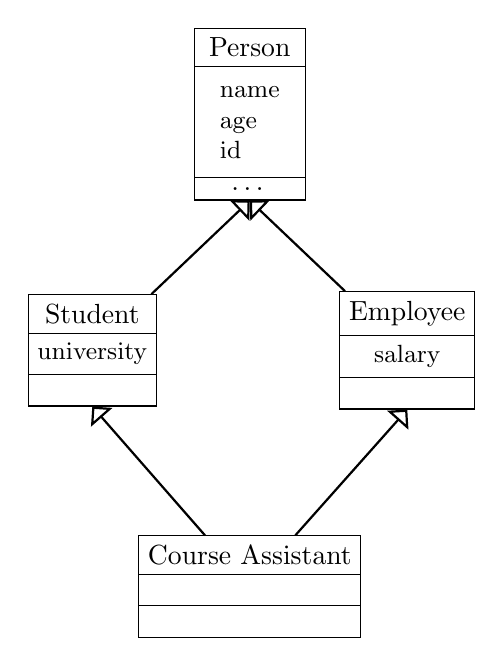
\begin{tikzpicture}
  \node[draw, rectangle split, rectangle split parts=3] (Person)   at
  (0,3) {Person \nodepart{second}\small \begin{tabular}{l}name\\
      age\\ id\end{tabular}
    \nodepart{third}
    \ldots
 };
\node[draw, rectangle split, rectangle split parts=3] (Student)  at (-2,0){Student
    \nodepart{second} \small university
 };
  \node[draw, rectangle split, rectangle split parts=3] (Employee) at
  (2,0) {Employee
    \nodepart{second} \small salary    
  };
  \node[draw, rectangle split, rectangle split parts=3] (CA) at (0,-3) {Course Assistant}; 
\draw[thick, open triangle 90-] (Person.south) -- (Student);
 \draw[thick, open triangle 90-] (Student.south) -- (CA);
 \draw[thick, open triangle 90-] (Person.south) -- (Employee);
 \draw[thick, open triangle 90-] (Employee.south) -- (CA);
\end{tikzpicture}
\end{minipage}
\begin{minipage}{0.49\textwidth}\small
  \begin{block}{Shared Inheritance}
    A child object contains \emph{only one} superclass object.
  \end{block}
  
Avoids name clashes between parents.\pause

\Blue{What if \texttt{Student} and \texttt{Employee} override
a method in \texttt{Person}?}\pause\\{\small Eiffel: \texttt{select}; \Cpp: Error }
\pause

Further Problems:
\begin{itemize}\small
\item In \Cpp, neither child nor virtual parent determine the construction
of parent objects---only grandchildren.
%\item In \Cpp, virtual function table gets either bigger or there is an additional level of indirection.
\item In Eiffel: it depends on the future client whether
a feature will be shared or replicated.
\end{itemize}\pause
$\leadsto$ \alert{Implementation quite complicated}
\end{minipage}
\end{frame}

\begin{frame}
\frametitle{Interfaces}
\framesubtitle{}
\hfill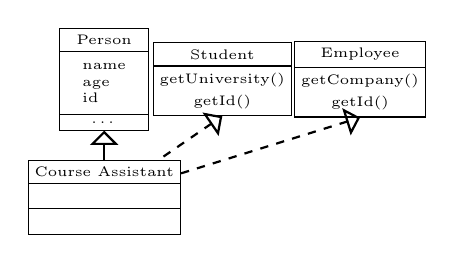
\begin{tikzpicture}\tiny
  \node[draw, rectangle split, rectangle split parts=3] (Person)   at
  (0,0) {Person \nodepart{second} \begin{tabular}{l}name\\
      age\\ id\end{tabular}
    \nodepart{third}
    \ldots
 };
\node[draw, rectangle split, rectangle split parts=2] (Student)  at (1.5,0) {Student
    \nodepart{second}  \shortstack{getUniversity() \\ getId()}
 };
  \node[draw, rectangle split, rectangle split parts=2] (Employee) at (3.25,0) {Employee
    \nodepart{second}  \shortstack{getCompany() \\ getId() }
  };
  \node[draw, rectangle split, rectangle split parts=3] (CA) at (0,-1.5) {Course Assistant}; 
\draw[thick, open triangle 90-] (Person.south) -- (CA);
 \draw[thick, dashed, open triangle 90-] (Student.south) -- (CA);
\draw[thick, dashed, open triangle 90-] (Employee.south) -- (CA);
\end{tikzpicture}

\vspace*{-5em}
Interfaces 
\begin{itemize}
  \item<+-> have no state
  \item<+-> contain only method declarations \\
    without providing an implementation
  \item<+-> complex subtyping while avoiding most problems of
    full-fledged multi-inheritance
\end{itemize}

\onslide<+->
\alert{but}

\begin{itemize}
  \item<+-> \emph{no} code reuse
  \item<+-> still problem when two interfaces declare same method which
    should have different semantics, e.g., \texttt{getId()} return
    student id resp.\ company id 
\end{itemize}
\onslide<+->
\Blue{Example:}\ interfaces in Java and C\#
\end{frame}


\begin{frame}[fragile]
\frametitle{Mix-ins}
\framesubtitle{}

\only<1|handout:0>{Interfaces nice, but can we improve on code reuse?\medskip}

\pause

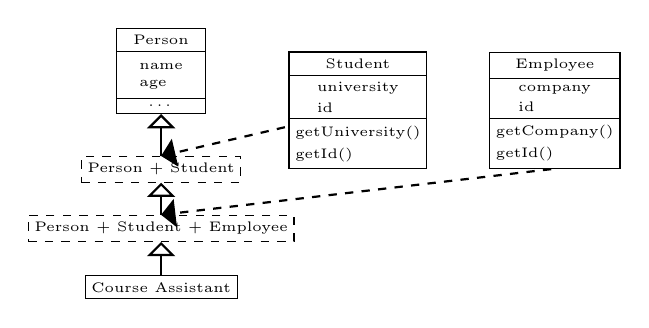
\begin{tikzpicture}\tiny
  \node[draw, rectangle split, rectangle split parts=3] (Person)   at
  (0,0.5) {Person \nodepart{second} \begin{tabular}{l}name\\
      age \end{tabular}
    \nodepart{third}
    \ldots
 };
\node[draw, rectangle split, rectangle split parts=3] (Student)  at (2.5,0) {Student
   \nodepart{second} \shortstack[l]{university \\ id  } \nodepart{third}  \shortstack[l]{getUniversity() \\ getId()}
 };
  \node[draw, rectangle split, rectangle split parts=3] (Employee) at (5,0) {Employee
    \nodepart{second} \shortstack[l]{company \\ id   }  \nodepart{third}  \shortstack[l]{getCompany() \\ getId()}
  };
  \node[draw, dashed, rectangle split, rectangle split parts=1] (PS) at (0,-0.75) {Person + Student}; 
  \node[draw, dashed, rectangle split, rectangle split parts=1] (PSE) at (0,-1.5) {Person + Student + Employee}; 
  \node[draw, rectangle split, rectangle split parts=1] (CA) at (0,-2.25) {Course Assistant}; 
\draw[thick, open triangle 90-] (Person.south) -- (PS);
\draw[thick, open triangle 90-] (PS.south) -- (PSE);
\draw[thick, open triangle 90-] (PSE.south) -- (CA);
\draw[thick, dashed, triangle 90-] (PS.north) -- (Student);
\draw[thick, dashed, triangle 90-] (PSE.north) -- (Employee.south) ;
\end{tikzpicture}
\medskip
\begin{overlayarea}{\textwidth}{0.5\textheight}
\only<2|handout:1>{
\Blue{Mix-ins} (here: \texttt{Student} and \texttt{Employee})
\begin{itemize}
\item have a state component, i.e., fields
\item define methods
\item define a type and organised in flat hierachy (no super- or
  submixins)
\item cannot be instantiated
\end{itemize}
}\only<3|handout:2>{
\Blue{Composition of Mix-ins}
\begin{itemize}
\item Mix-ins are \emph{mixed} into a class which is then referred to
  as mixee (here: Course Assistant)
\item Mixing follows linear order; superclass overides all
  mix-ins; within mix-ins most right overrides left;
  here student's \texttt{getId()} overrides employee's
\item Fields: if field of same name and type exists unified otherwise inherited
\end{itemize}
}\only<4|handout:3>{%
\Blue{Problems and Restrictions}
\begin{itemize}
\item Mixee has not full control over composition (cannot access all
  implementations of \texttt{getId()})
\item Adding method to one mix-in can silently change behavior of a
  completely unrelated mixee (because of implicit conflict resolution)
\item Mix-ins cannot be combined to new mix-ins
\end{itemize}
}
\end{overlayarea}
\end{frame}

\begin{frame}[fragile]
\frametitle{Traits}
\only<1|handout:1>{Can we do even better?} \pause 

\begin{center}
\begin{overlayarea}{0.6\textwidth}{0.3\textheight}
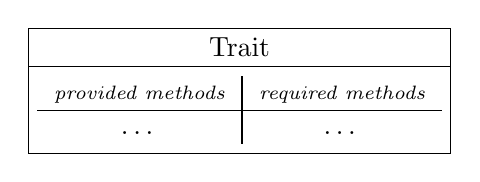
\begin{tikzpicture}
  \node[draw, rectangle split, rectangle split parts=2] (trait) at
  (0,0) { Trait \nodepart{second} 
    \begin{tabular}{c|c}\scriptsize
      \it provided  methods  & \scriptsize\it required methods \\ \hline
    \ldots &  \ldots 
  \end{tabular}  };
\end{tikzpicture}
\end{overlayarea}
\end{center}

\begin{overlayarea}{\textwidth}{0.68\textheight}
\only<2|handout:2>{%
\begin{definition}[Trait]
  A \emph{trait} is solely a \emph{unit of reuse} and does \emph{not}
  declare a nominal type. A trait consists of a set of provided
  methods and a set of required methods.
\end{definition}
}\only<3|handout:3>{%
  \Blue{Trait Facts}
  \begin{itemize}
    \item traits are \emph{not} types
    \item traits have \emph{no} state $\Rightarrow$ provided methods
      cannot access the internal state (have to go via required
      methods)
    \end{itemize}%
}\only<4|handout:4>{%
  \Blue{Trait Composition: Class = State + Superclass + Traits + Glue}
  \begin{itemize}    
  \item Conflicts must be resolved manually 
  \item Number of trait composition operators: union, exclusion (turns
    a provided method into a required method), renaming etc.
  \item Client class \emph{using} traits maintains control
  \item Traits can be composed to new traits
  \item Flattening: after composition class has same semantics as if
    methods would have been implemented directly
\end{itemize}}
\end{overlayarea}
\end{frame}

\section{Simulating Multi-Dispatch}

\subsection{Dispatch Semantics}
\begin{frame}[fragile]
\frametitle{Recall: Method Dispatching}
\framesubtitle{}

Single-dispatch languages
\begin{itemize}
\item Dispatch based on the (dynamic) class of the receiver. 
\begin{cplus3}
     Complex c = ... ;   
     c.add(arg);
\end{cplus3}
\item Ex.: all languages mentioned so far

\end{itemize}

Multiple-dispatch languages
\begin{itemize}
\item Dispatch (also) based on the dynamic class of \textit{arguments}.
\item Ex.: Dylan (Apple), CLOS, Cecil
\end{itemize} 
\end{frame}


\subsection{Overriding in real languages}

\begin{frame}[fragile]
\frametitle{Overriding rules in real languages}
\framesubtitle{}
Overriding can be \textit{covariant}, 
\textit{contravariant}, or \textit{invariant} in either
the argument types or the return type.
\bigskip


Assume a class \texttt{Animal}, a child \texttt{DomesticAnimal} with 
%a method 
%\begin{center} set_playmate(Sandwich) → void \end{center}
\begin{cplus3}
       set_playmate(DomesticAnimal)->  void 
\end{cplus3}

and the child \texttt{Cat},
which re-defines \texttt{set_playmate}. 
How may the argument type change?% (relativeto DomesticAnimal.set_playmate):
\begin{itemize}
\item Covariance (in the argument type):
\begin{cplus3}
 set_playmate(Cat) -> void
\end{cplus3}
 \item Contravariance:
\begin{cplus3}
 set_playmate(Animal) -> void
\end{cplus3}
  \item Invariance: 
\begin{cplus3}
 set_playmate(DomesticAnimal) -> void
\end{cplus3}


\end{itemize}
Eiffel uses the covariance rule; but this can be unsafe (why?).
%http://www.faqs.org/faqs/eiffel-faq/
Most languages use the invariance rule (for argument types). 
\end{frame}

\begin{frame}[fragile]
\frametitle{Covariance in return type}
\framesubtitle{}
Covariance in the return type is less contested.
\bigskip

\begin{cplus3}
// Java 1.5
class BaseClass {
    public BaseClass Clone() {..}
}
class DerivedClass extends BaseClass {
    public DerivedClass Clone() {..}
}
\end{cplus3}
Java, \Cpp, Eiffel support covariance in the return type.\\
C\# requires invariance. 
\end{frame}

\begin{frame}[fragile]{Double-Disptach in a Single-Dispatch Language}

How? \pause \alert{Visitor Pattern}

\bigskip

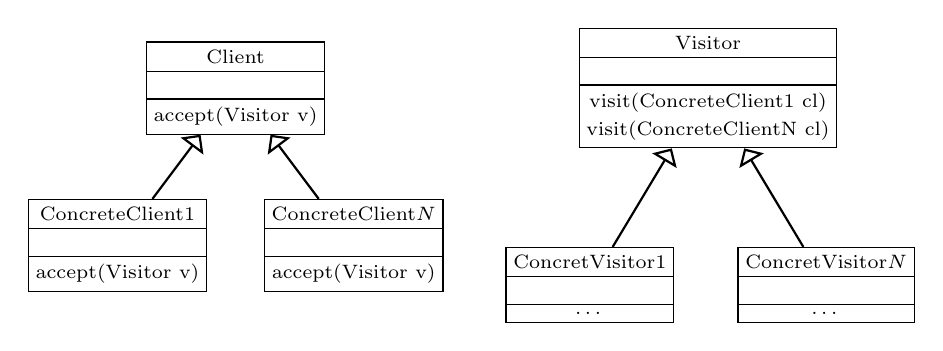
\begin{tikzpicture}\scriptsize

\node[draw, rectangle split, rectangle split parts=3] (Client) at (0,0) {Client \nodepart{second} \nodepart{third} accept(Visitor v) };

\node[draw, rectangle split, rectangle split parts=3] (CC1) at (-1.5,-2) {ConcreteClient$1$ \nodepart{second} \nodepart{third} accept(Visitor v) };
\node[draw, rectangle split, rectangle split parts=3] (CCN) at (1.5,-2) {ConcreteClient$N$ \nodepart{second} \nodepart{third} accept(Visitor v) };

\draw[open triangle 90-, thick] (Client) -- (CC1);
\draw[open triangle 90-, thick] (Client) -- (CCN);


\node[draw, rectangle split, rectangle split parts=3] (Visitor) at (6,0) {Visitor \nodepart{second} \nodepart{third}
  \shortstack{visit(ConcreteClient1 cl) \\ visit(ConcreteClientN cl)}};
\node[draw, rectangle split, rectangle split parts=3] (CV1) at (4.5,-2.5) {ConcretVisitor$1$ \nodepart{second} \nodepart{third} \ldots};
\node[draw, rectangle split, rectangle split parts=3] (CVN) at (7.5,-2.5) {ConcretVisitor$N$ \nodepart{second} \nodepart{third} \ldots};

\draw[open triangle 90-, thick] (Visitor) -- (CV1);
\draw[open triangle 90-, thick] (Visitor) -- (CVN);

\end{tikzpicture}


\pause

\Blue{Usage}

\begin{java}
ConcreteClient1::accept(Visitor v) { v.visit(this); }
 
ConcreteClientN::accept(Visitor v) { v.visit(this); }

Visitor v;  Client cl;
...
cl.accept(v);
\end{java}

\end{frame}



\end{document}